\section{巧求周长(一)}

\title[第1讲\quad 巧求周长(一)]{第1讲\quad 巧求周长(一)} 
\author{}
\date{}
\begin{frame}
    \titlepage
\end{frame}

% \subsection{课前测}
\begin{frame}
    \frametitle{课前测}
    \begin{figure}[H] %H为当前位置,!htb为忽略美学标准,htbp为浮动图形
        \centering %图片居中
        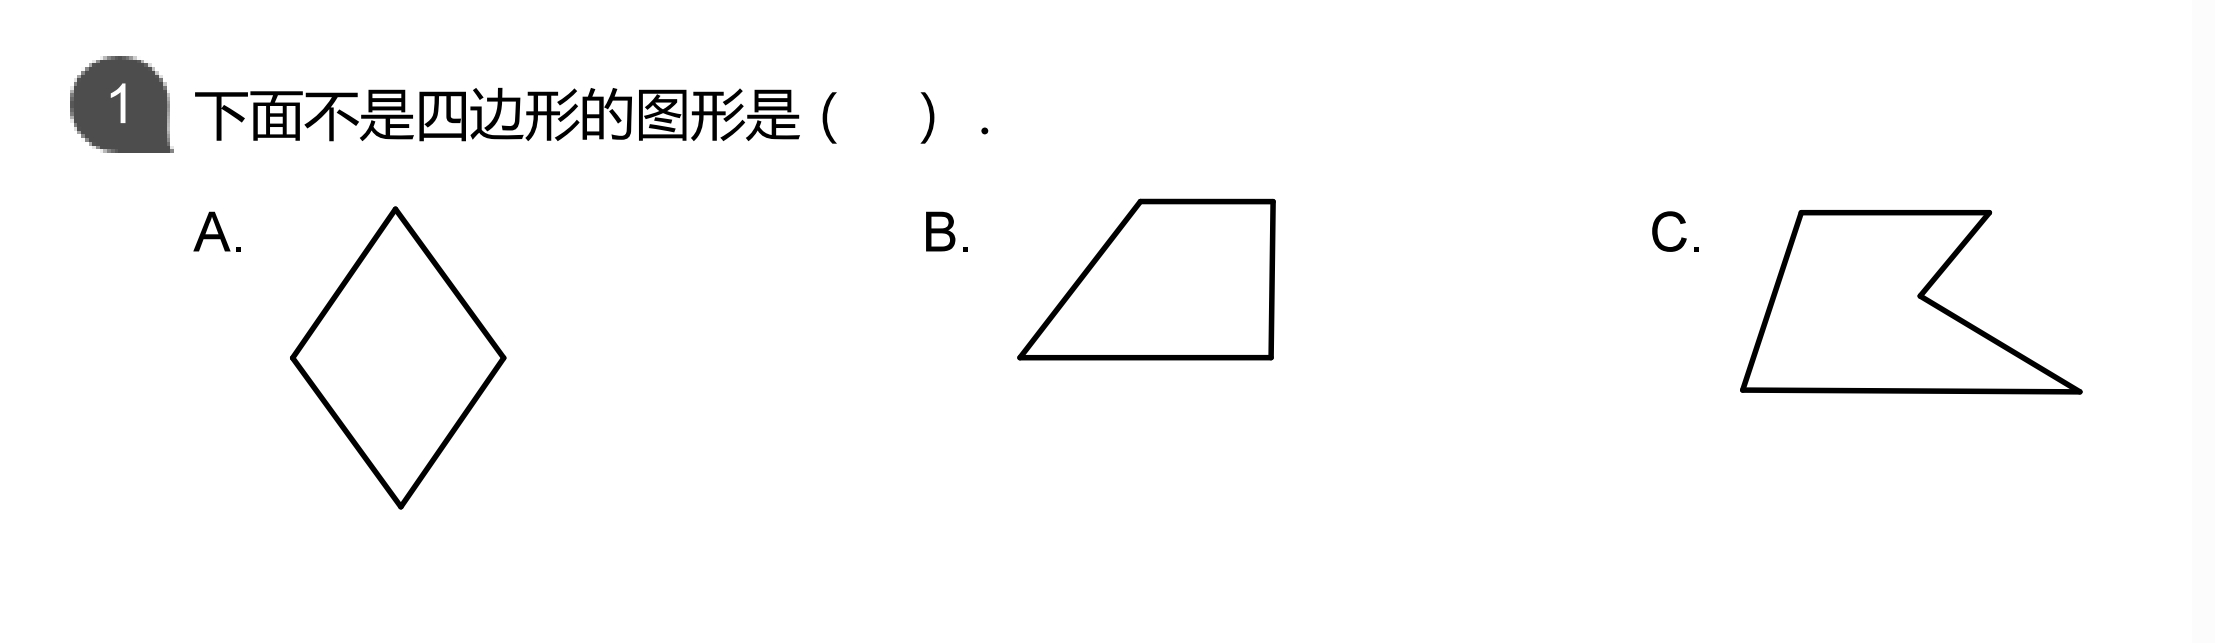
\includegraphics[width=1\textwidth]{./pics/Chapter_1/1.png} %插入图片,[]中设置图片大小,{}中是图片文件名
        % \caption{} % 显示图片标题
        % \label{Fig.main2} %用于文内引用的标签
    \end{figure}
    
    % \rightline{Posted outside the mathematics reading room,Tromso University}
\end{frame}

\begin{frame}
    \frametitle{课前测}
    \begin{figure}[H] 
        \centering
        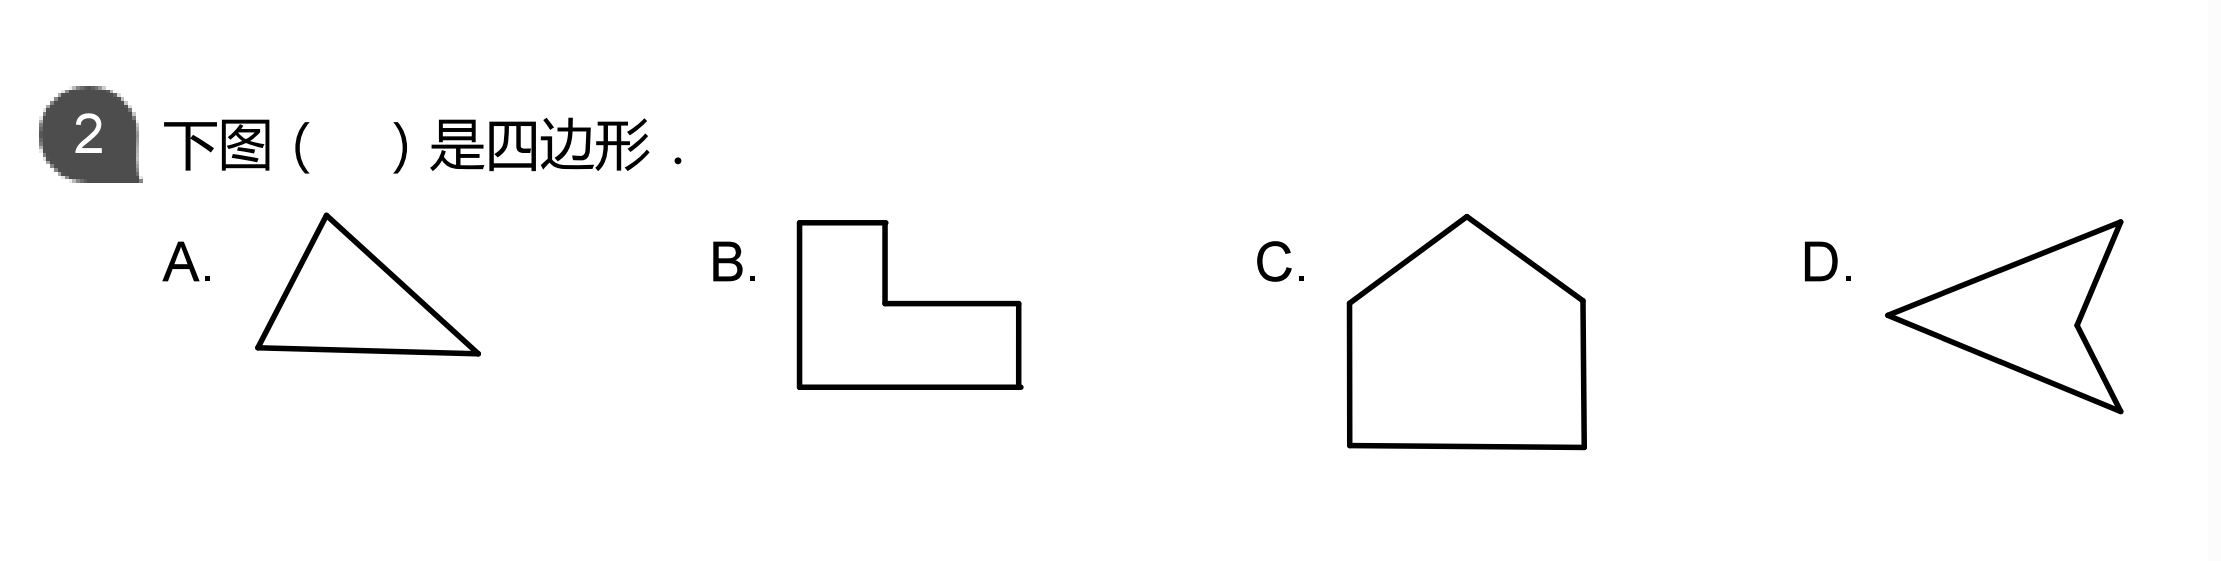
\includegraphics[width=1\textwidth]{./pics/Chapter_1/2.png}
    \end{figure}
\end{frame}

\begin{frame}
    \frametitle{课前测}
    \begin{figure}[H] 
        \centering
        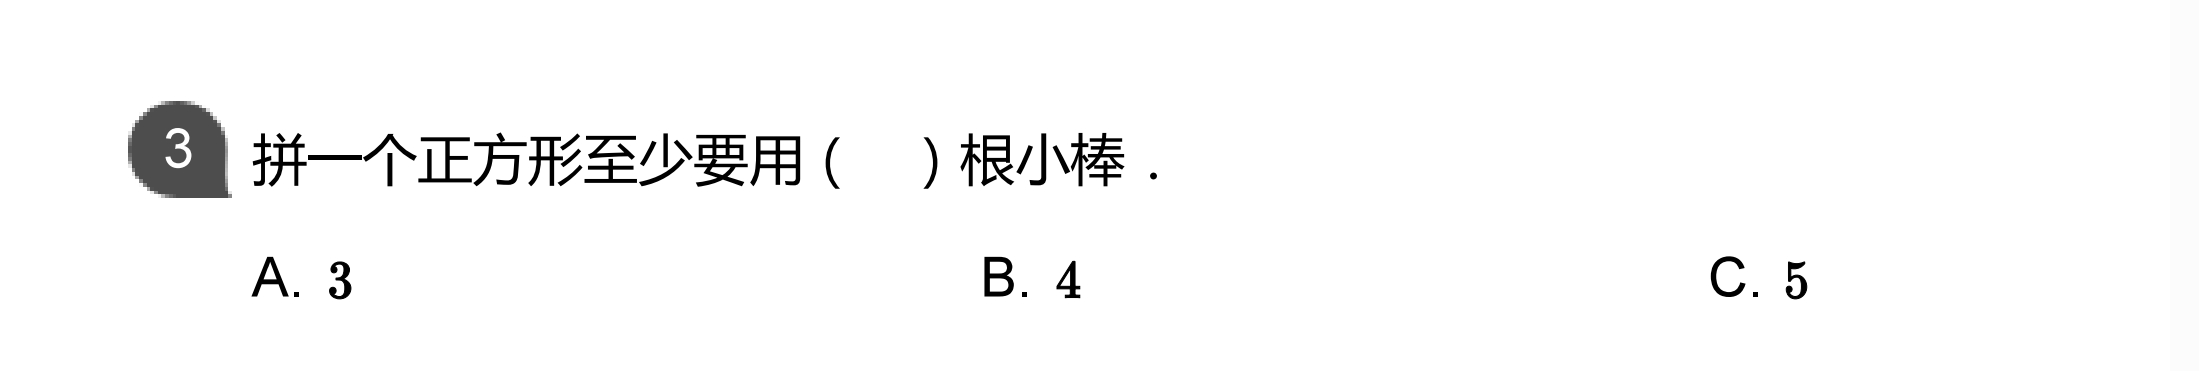
\includegraphics[width=1\textwidth]{./pics/Chapter_1/3.png}
    \end{figure}
\end{frame}

% \subsection{知识梳理}
\begin{frame}
    \frametitle{知识梳理}
\end{frame}

% \subsection{MISSION 1}
\begin{frame}
    \frametitle{MISSION 1}
    \begin{figure}[H] 
        \centering
        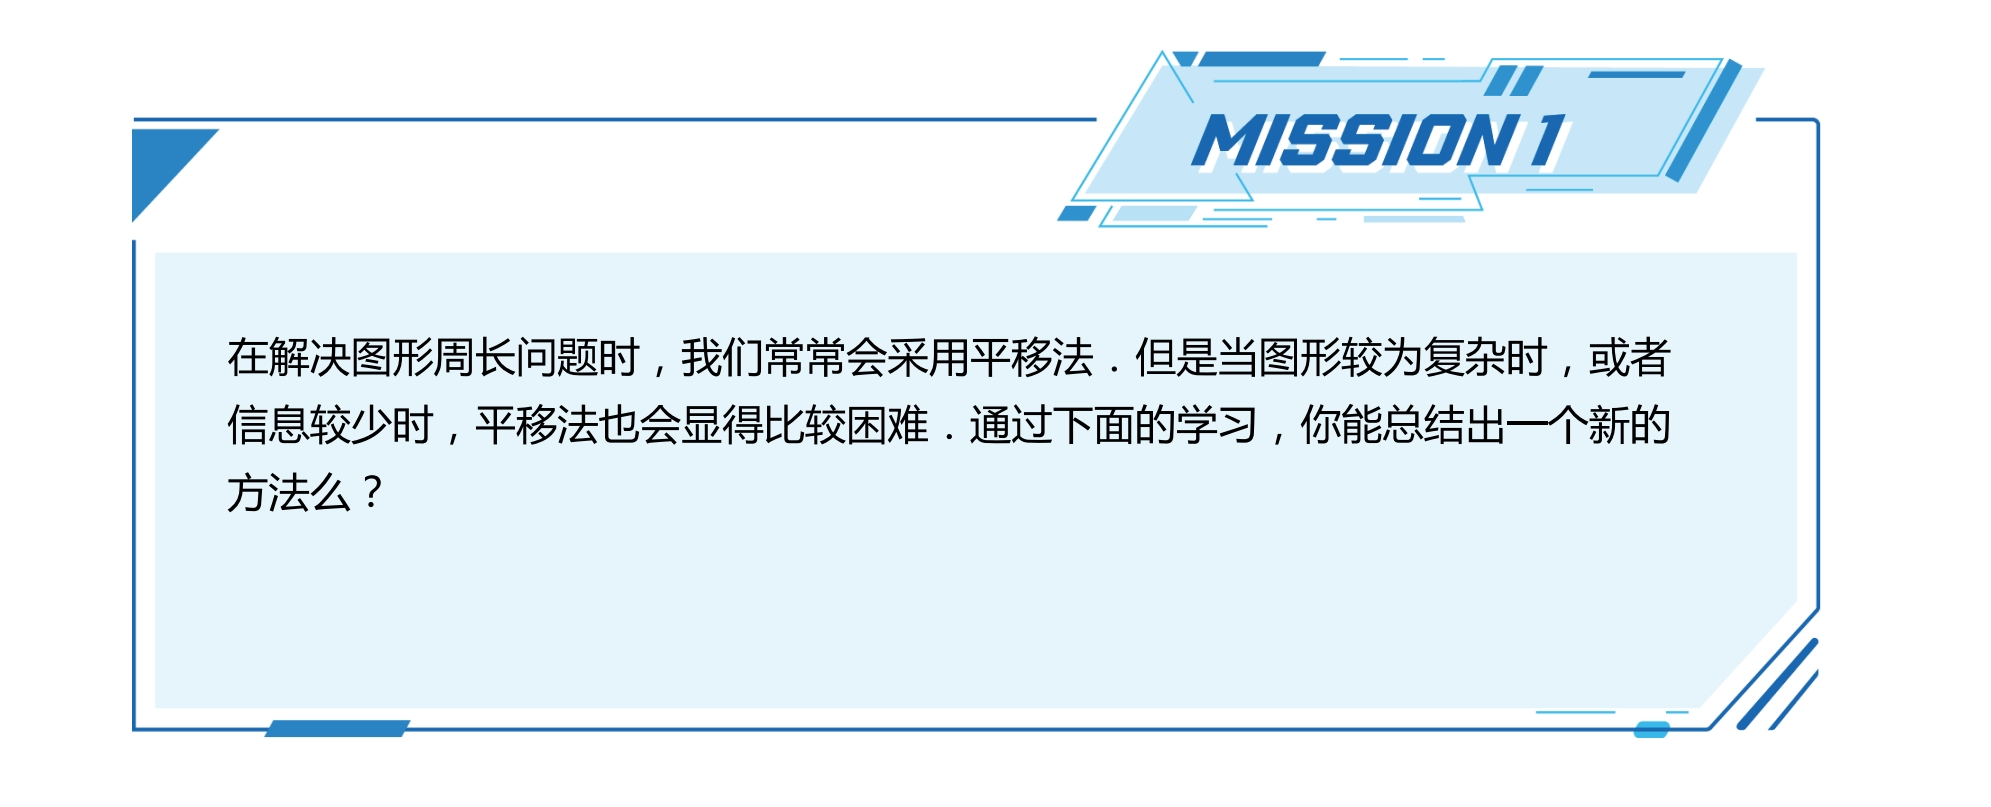
\includegraphics[width=1\textwidth]{./pics/Chapter_1/mission1.png}
    \end{figure}
\end{frame}

% \subsection{探索1}
\begin{frame}
    \frametitle{探索1}
    \begin{figure}[H] 
        \centering
        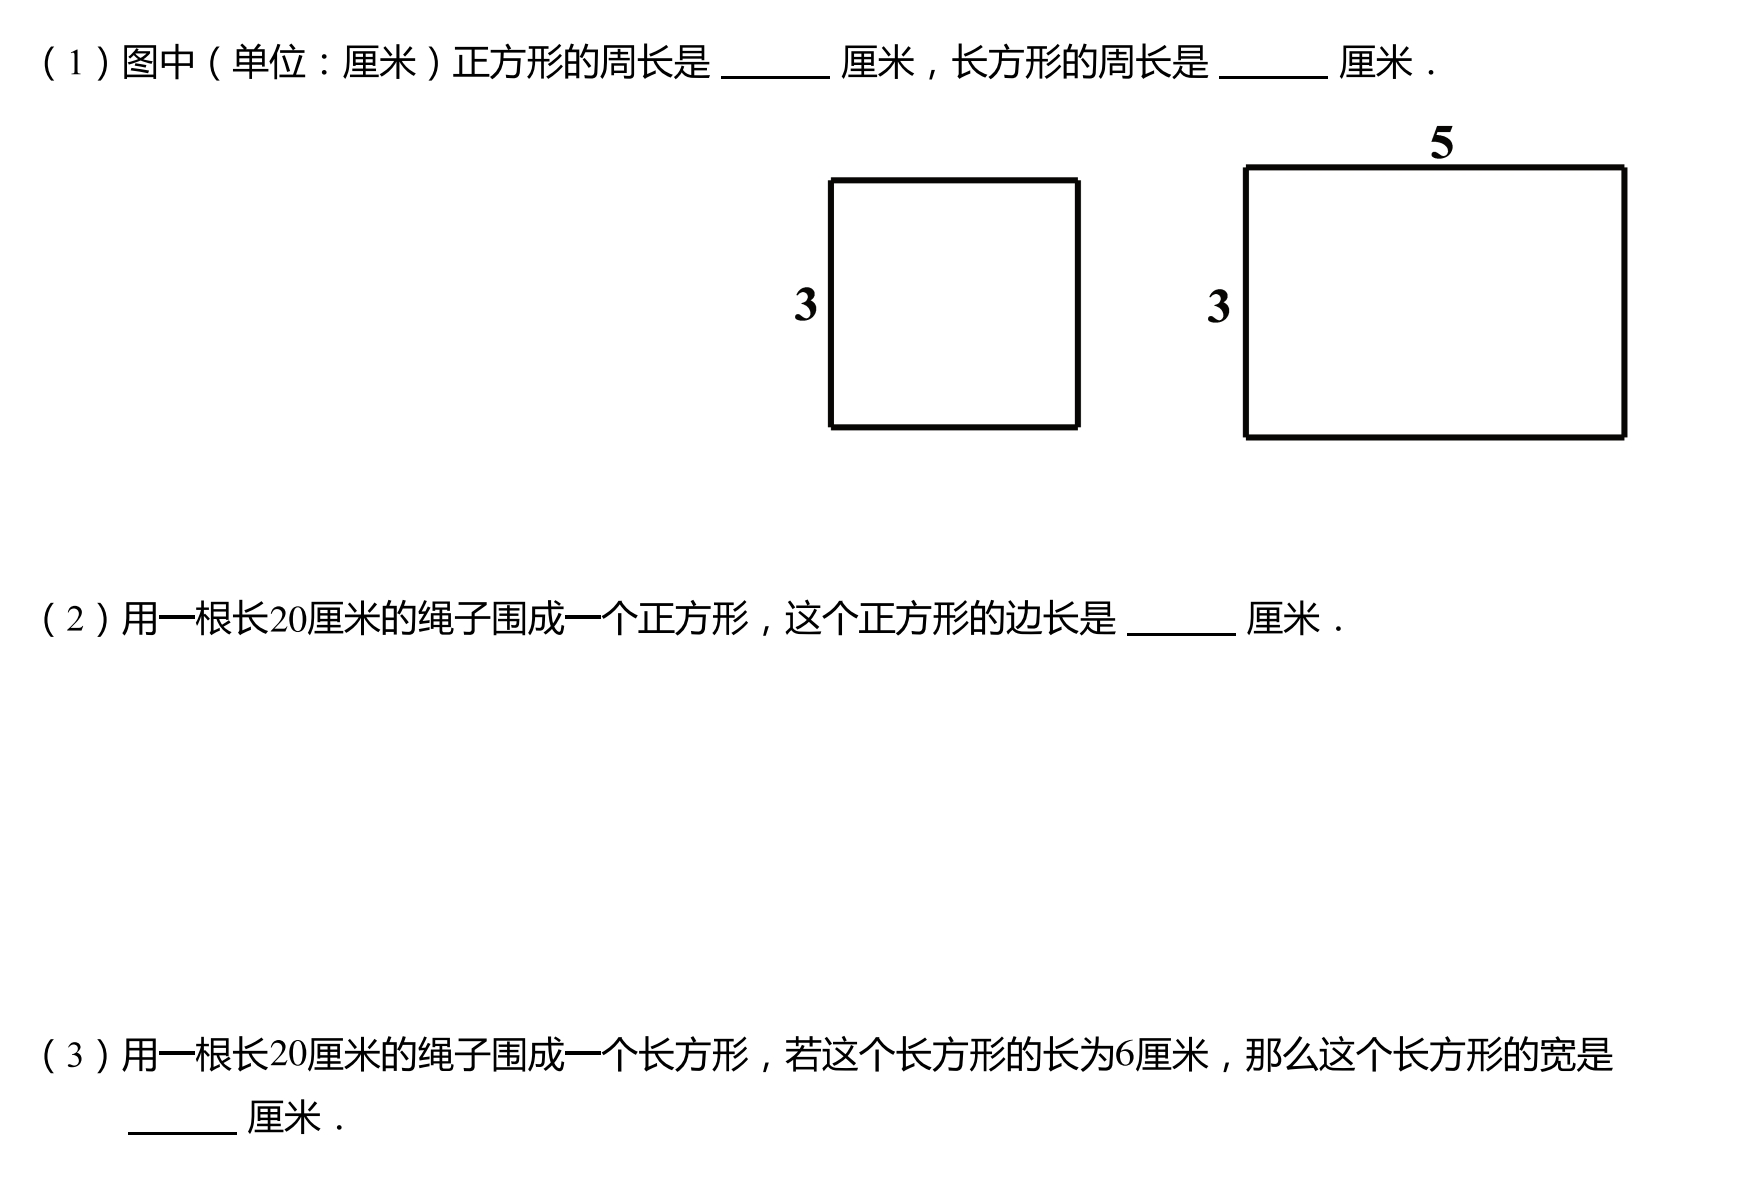
\includegraphics[width=0.8\textwidth]{./pics/Chapter_1/tansuo1.png}
    \end{figure}
\end{frame}

\begin{frame}
    \frametitle{铺垫1}
    \textit{俄尔金正在研制一种仿生蚂蚁机器人,希望窃取超能先锋的情报:下图是一个长宽分别为60厘米和50厘米的长方形,在该地形上对蚂蚁机器人进行测试.甲、乙两只小蚂蚁同时从左上角出发,以同样的速度分别沿图中虚线爬行到达B点,问:哪只蚂蚁先到达?两只蚂蚁共爬行了多少路程?}
    \begin{figure}[H] 
        \centering
        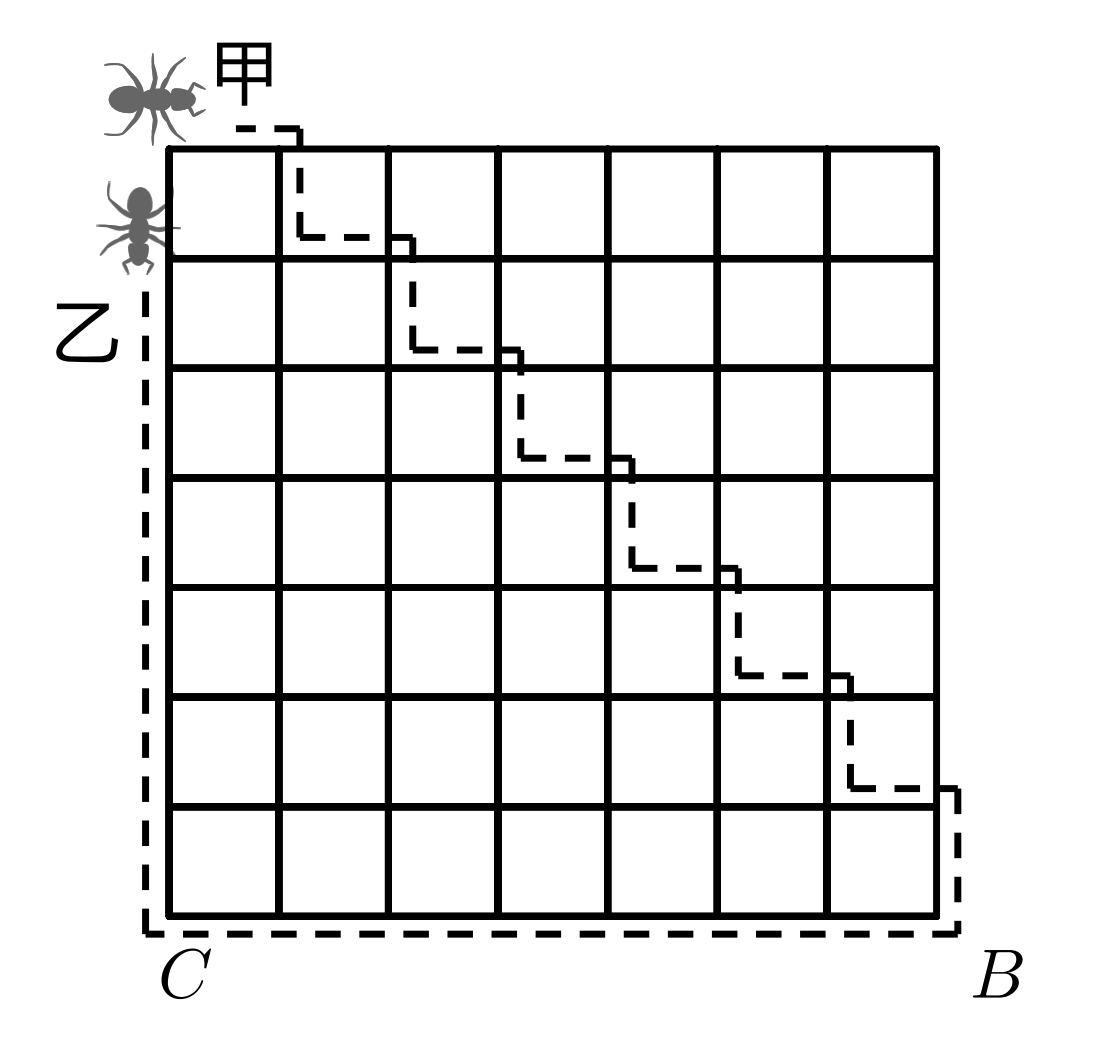
\includegraphics[width=0.4\textwidth]{./pics/Chapter_1/pudian1.png}
    \end{figure}
\end{frame}

\begin{frame}
    \frametitle{探索2}
    \textit{俄尔金正在研制一种仿生蚂蚁机器人,希望窃取超能先锋的情报,博士知道此事后,为了加强安全,正在加紧制作一个精密仪器,检测蚂蚁机器人的潜入.为了保证仪器精准,需要对核心零件进行测量.请你帮助博士测量下面核心零件的周长.(单位:厘米)}
    \begin{figure}[H] 
        \centering
        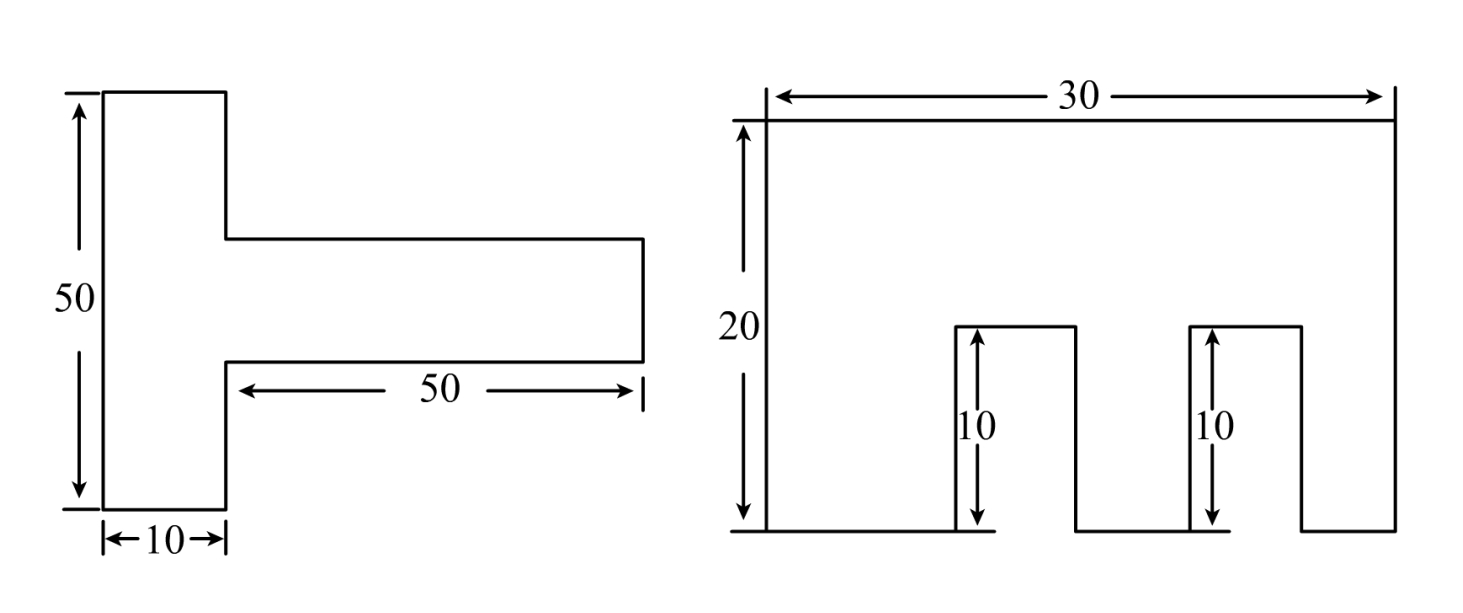
\includegraphics[width=1\textwidth]{./pics/Chapter_1/tansuo2.png}
    \end{figure}
\end{frame}

\begin{frame}
    \frametitle{探索2}
    \textit{在你的帮助下,博士的精密仪器终于研制完成.仪器的侧面平面图如下,图中每一条最短线段的长为5厘米,这个零件高30厘米,这个仪器侧面的周长是多少厘米?}
    \begin{figure}[H] 
        \centering
        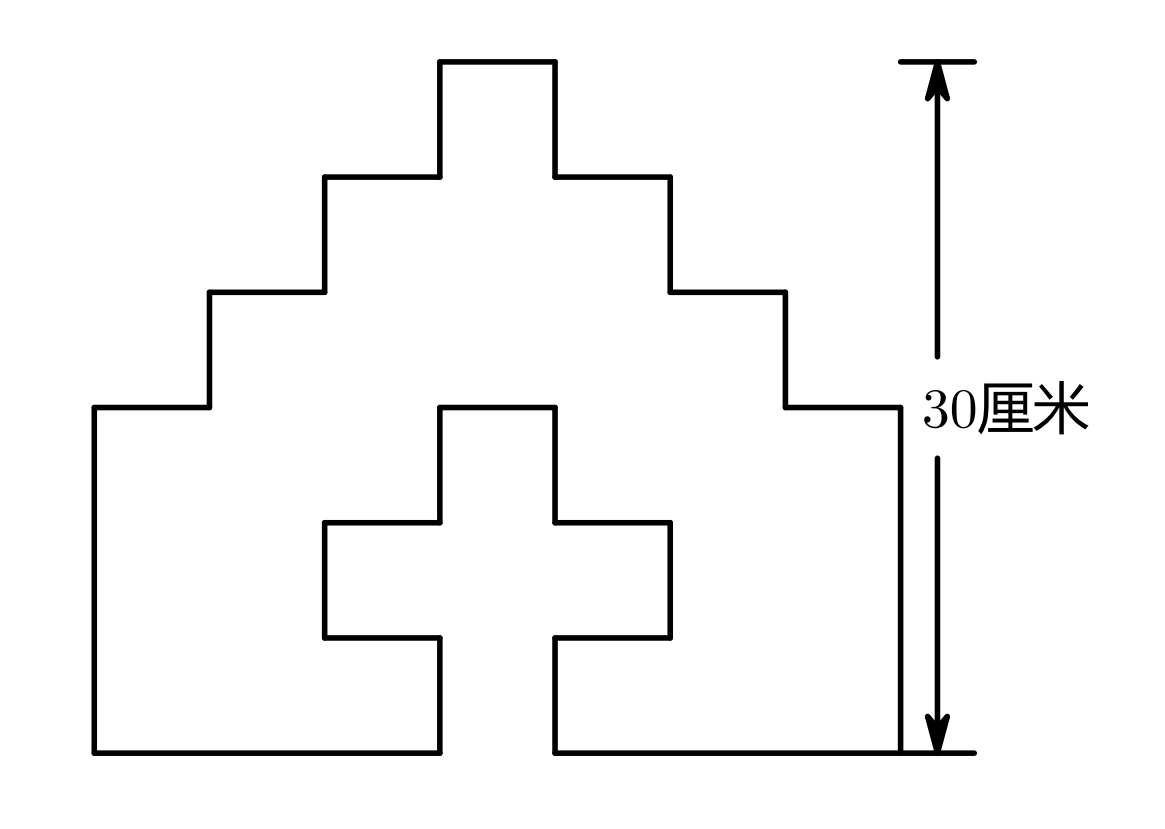
\includegraphics[width=0.5\textwidth]{./pics/Chapter_1/tansuo2_2.png}
    \end{figure}
\end{frame}

% \subsection{捉虫时刻}
\begin{frame}
    \frametitle{捉虫时刻}
    \begin{figure}[H] 
        \centering
        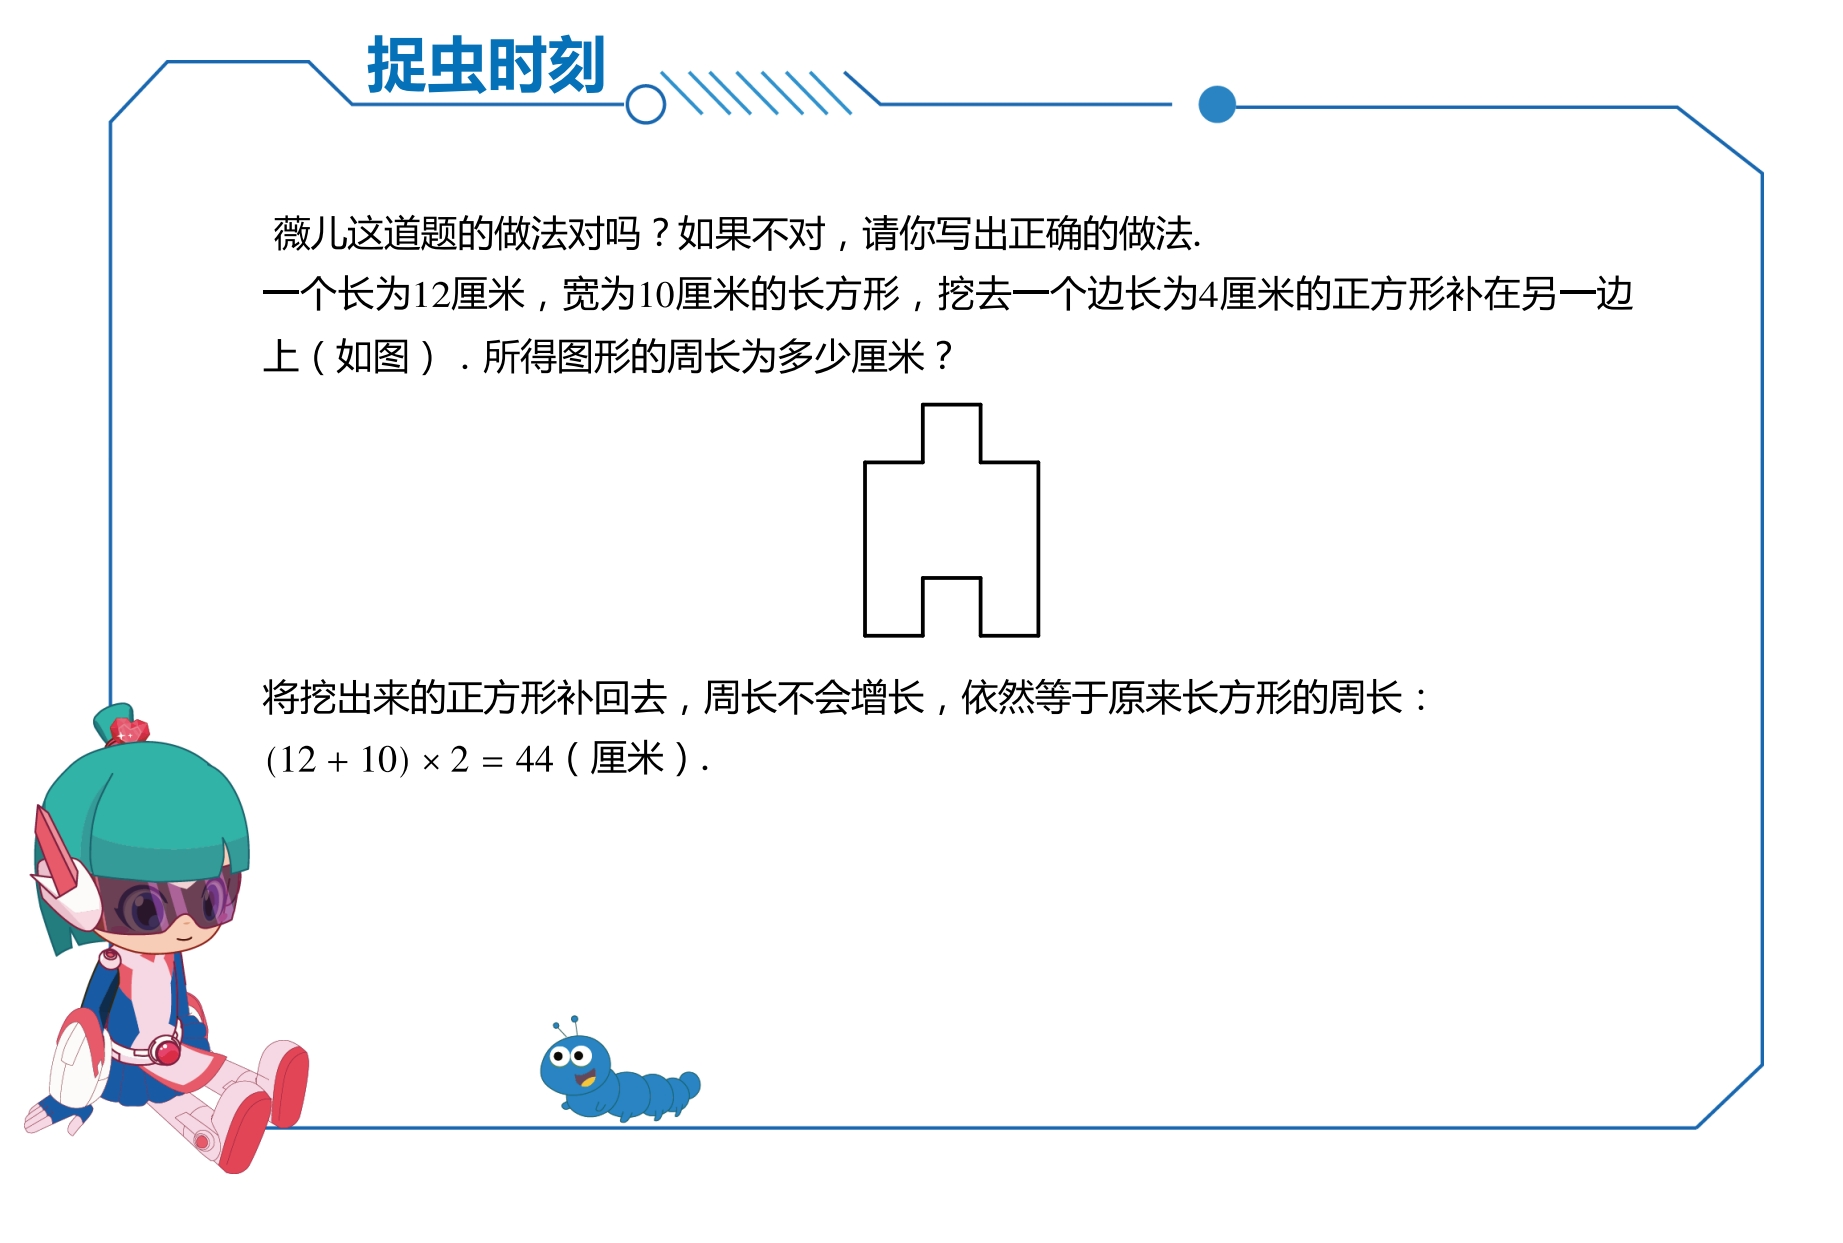
\includegraphics[width=1\textwidth]{./pics/Chapter_1/zhuochong1.png}
    \end{figure}
\end{frame}

% \subsection{探索3}
\begin{frame}
    \frametitle{探索3}
    \textit{除了被动防御措施,博士也研发了一种仿生机器人--A型食蚁兽.在一次测试中,A型食蚁兽经历多次向上、向下、向左、向右后回到出发点,路线形成一个缺角的山字形.请问它一共走了多少米?}
    \begin{figure}[H] 
        \centering
        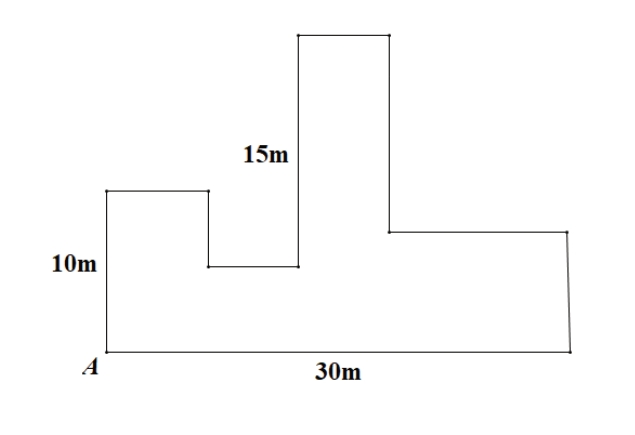
\includegraphics[width=0.5\textwidth]{./pics/Chapter_1/tansuo3.png}
    \end{figure}
\end{frame}

\begin{frame}
    \frametitle{课堂互动}
    \begin{figure}[H] 
        \centering
        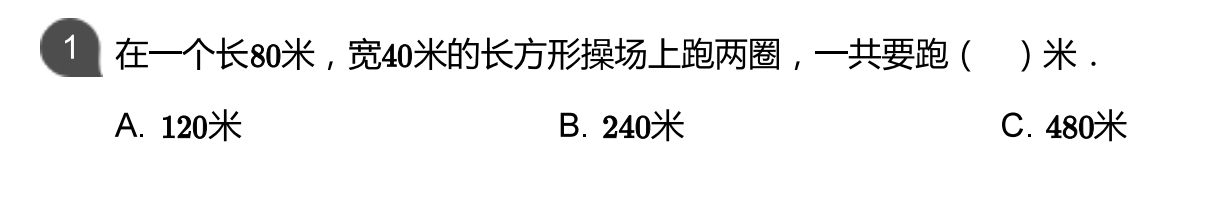
\includegraphics[width=1\textwidth]{./pics/Chapter_1/kthd1.png}
    \end{figure}
\end{frame}

\begin{frame}
    \frametitle{课堂互动}
    \begin{figure}[H] 
        \centering
        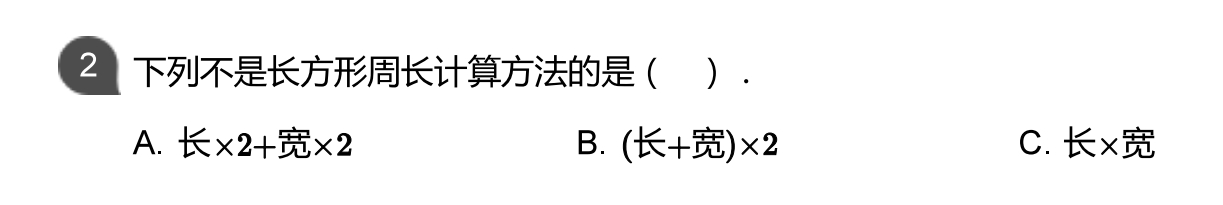
\includegraphics[width=1\textwidth]{./pics/Chapter_1/kthd2.png}
    \end{figure}
\end{frame}

\begin{frame}
    \frametitle{课堂互动}
    \begin{figure}[H] 
        \centering
        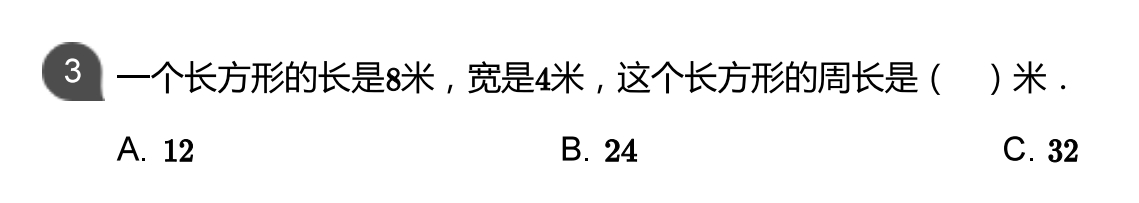
\includegraphics[width=1\textwidth]{./pics/Chapter_1/kthd3.png}
    \end{figure}
\end{frame}

% \subsection{探索4}
\begin{frame}
    \frametitle{探索4}
    \textit{一个边长为6厘米的正方形纸片,若沿边向内剪去一个边长是2厘米的小正方形,所剩图形的周长是多少厘米?}
\end{frame}

% \subsection{MISSION 2}
\begin{frame}
    \frametitle{MISSION 2}
    \begin{figure}[H] 
        \centering
        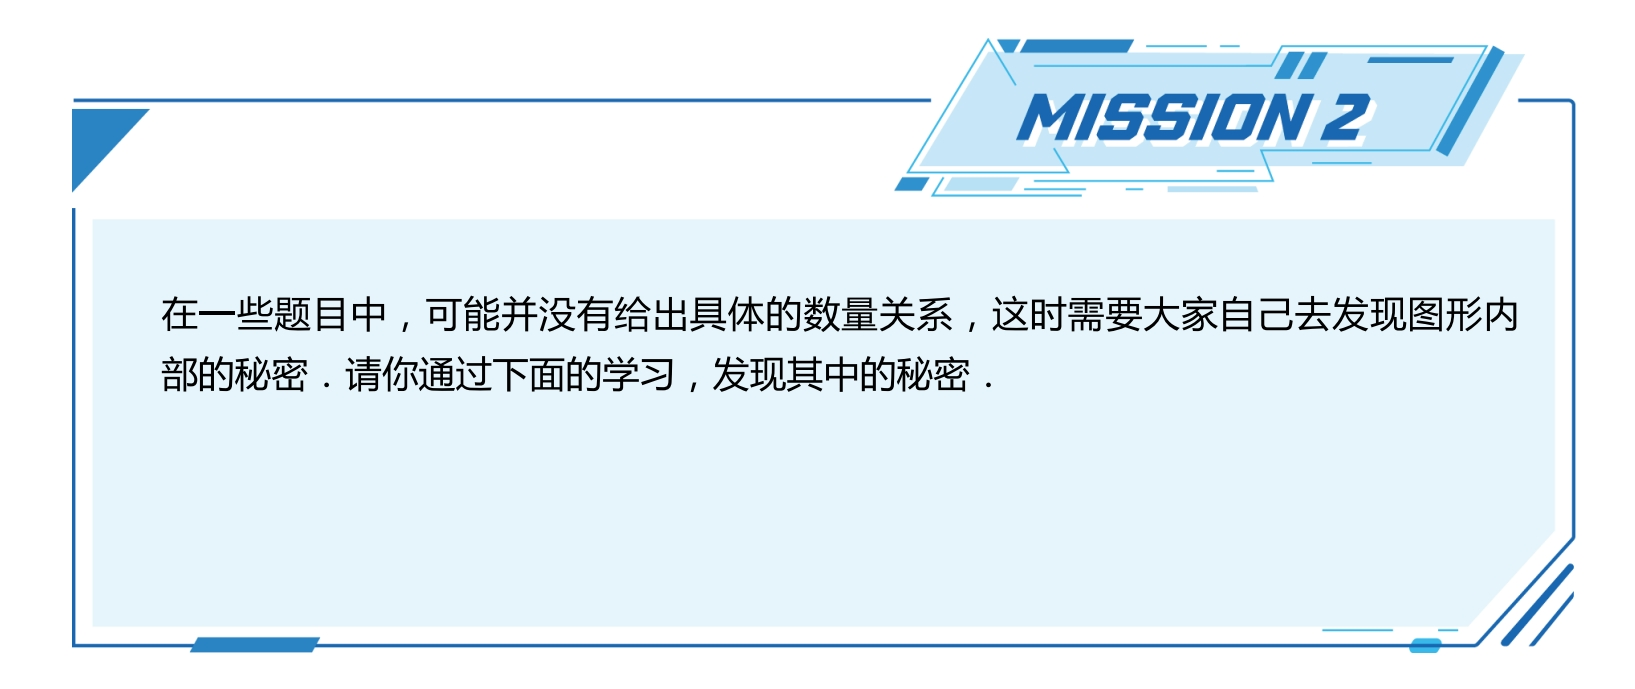
\includegraphics[width=1\textwidth]{./pics/Chapter_1/mission2.png}
    \end{figure}
\end{frame}

\begin{frame}
    \frametitle{铺垫2}
    \textit{如图,把一个大正方形分割成9个小正方形,这9个小正方形的周长之和是72厘米,原来大正方的周长是厘米?}
    \begin{figure}[H] 
        \centering
        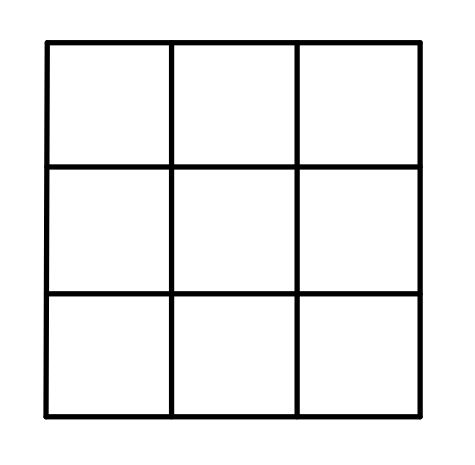
\includegraphics[width=0.5\textwidth]{./pics/Chapter_1/pudian2.png}
    \end{figure}
\end{frame}

% \subsection{探索5}
\begin{frame}
    \frametitle{探索5}
    \textit{(1)一张长方形纸片,如下图,先左右对折,再上下对折,再左右对折,再上下对折,折叠后的长方形纸片的周长是12厘米,折叠前的长方形纸片的周长是多少厘米?}
    \begin{figure}[H] 
        \centering
        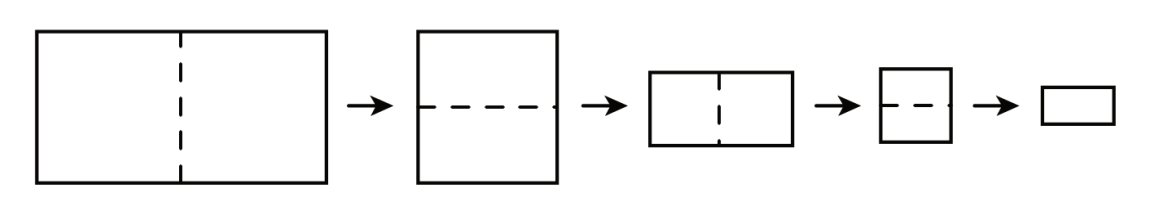
\includegraphics[width=1\textwidth]{./pics/Chapter_1/tansuo5.png}
    \end{figure}
\end{frame}

\begin{frame}
    \frametitle{探索5}
    \textit{(2)一个正方形纸片边长是12厘米,现将这张正方形纸片对折再对折,折叠后每个图形的周长可能是\underline{\hbox to 10mm{}}厘米,也可能是\underline{\hbox to 10mm{}}厘米}
\end{frame}

\begin{frame}
    \frametitle{铺垫3}
    \textit{把12个边长是1厘米的正方形纸拼成长方形.第( )种拼法拼成的图形周长最短}
    \begin{figure}[H] 
        \centering
        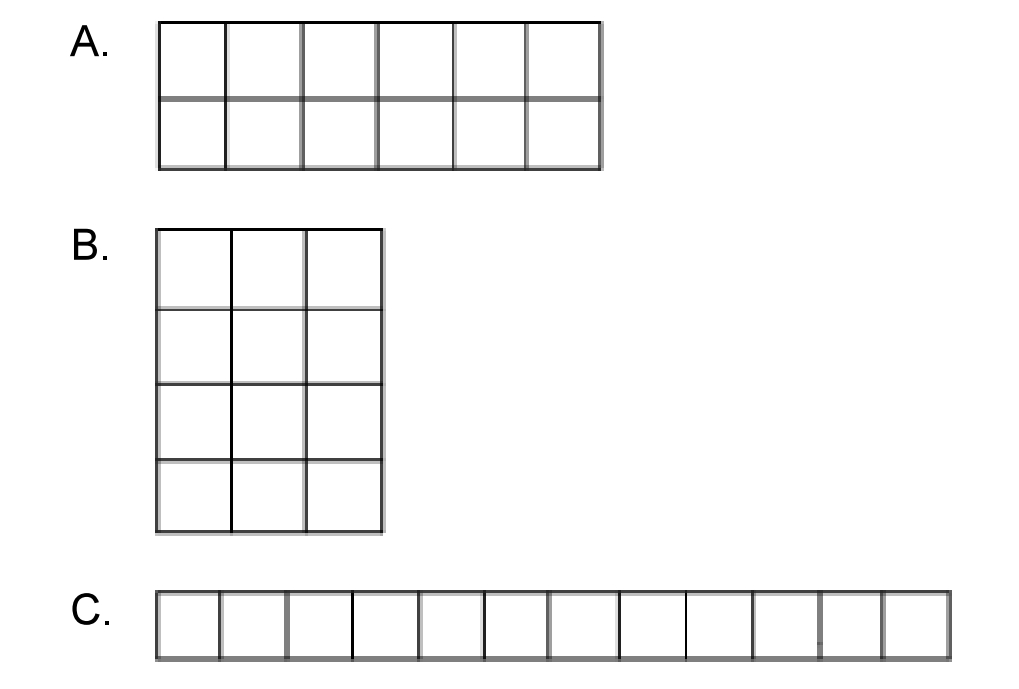
\includegraphics[width=0.5\textwidth]{./pics/Chapter_1/pudian3.png}
    \end{figure}
\end{frame}

% \subsection{探索6}
\begin{frame}
    \frametitle{探索6}
    \textit{用16张边长是3厘米的正方形纸拼长方形或正方形.怎样拼成的图形的周长最短?最短周长是多少
    厘米?}
\end{frame}

% \subsection{探索7}
\begin{frame}
    \frametitle{探索7}
    \textit{如图,求图中所有长方形的周长和}
    \begin{figure}[H] 
        \centering
        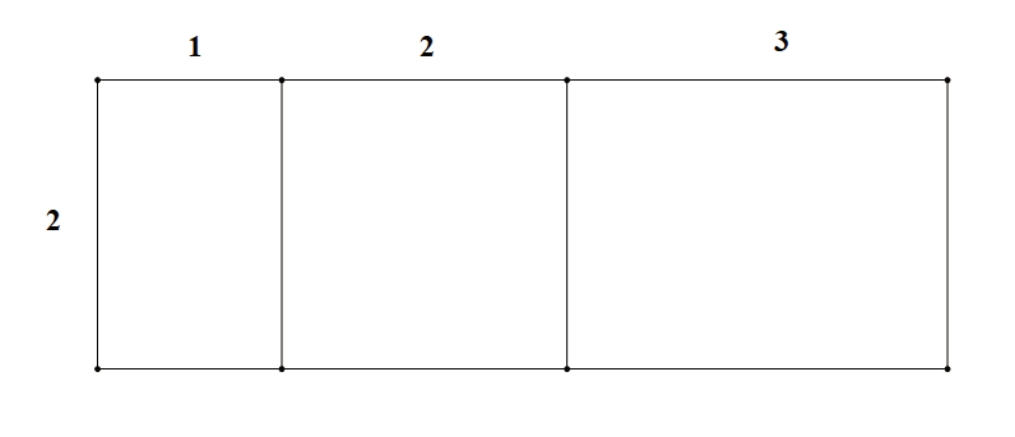
\includegraphics[width=0.8\textwidth]{./pics/Chapter_1/tansuo7.png}
    \end{figure}
\end{frame}

\begin{frame}
    \frametitle{铺垫4}
    \textit{一个长方形被分成了9小块,其中4块周长已经标出,则大长方形的周长为
    多少厘米}
    \begin{figure}[H] 
        \centering
        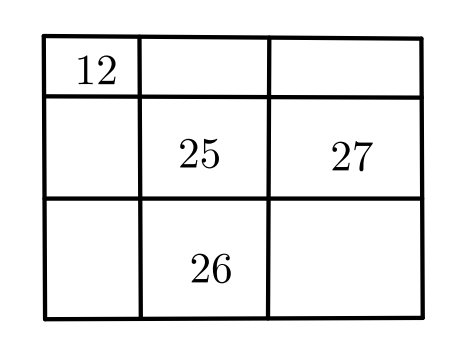
\includegraphics[width=0.5\textwidth]{./pics/Chapter_1/pudian4.png}
    \end{figure}
\end{frame}

% \subsection{探索8}
\begin{frame}
    \frametitle{探索8}
    \textit{(1)如图,将一个大长方形分割成9个小长方形.图上已标出部分小长方形的周长,那么阴影小长方形的周长是多少?}
    \begin{figure}[H] 
        \centering
        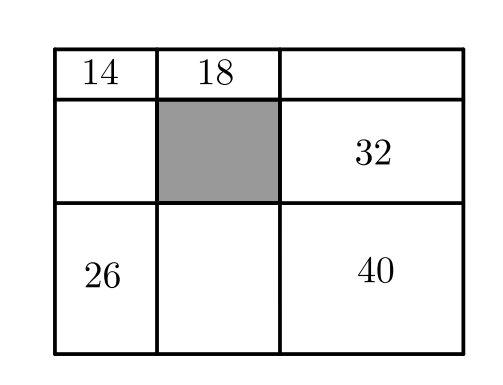
\includegraphics[width=0.5\textwidth]{./pics/Chapter_1/tansuo8_1.png}
    \end{figure}
\end{frame}

\begin{frame}
    \frametitle{探索8}
    \textit{(2)薇儿将一块大长方形地砖分成了9个小长方形,第一行3个小长方形与第一列3个小长方形的周长和为60,f与h的周长之和为20,那么这块地砖的周长是多少?}
    \begin{figure}[H] 
        \centering
        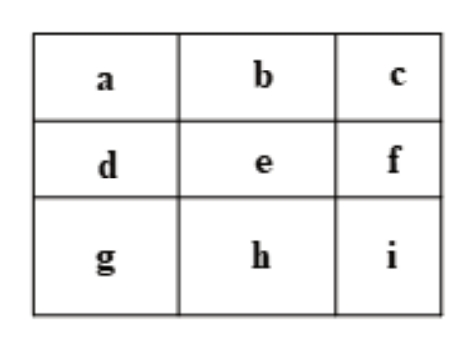
\includegraphics[width=0.5\textwidth]{./pics/Chapter_1/tansuo8_2.png}
    \end{figure}
\end{frame}

\begin{frame}
    \frametitle{补充1}
    \textit{将一张边长为12厘米的正方形纸对折,再将对折后的纸沿它的竖直中线(图中的虚线)虚线剪开,得到三个长方形纸片,其中两个较小的长方形的周长之和是多少厘米?}
    \begin{figure}[H] 
        \centering
        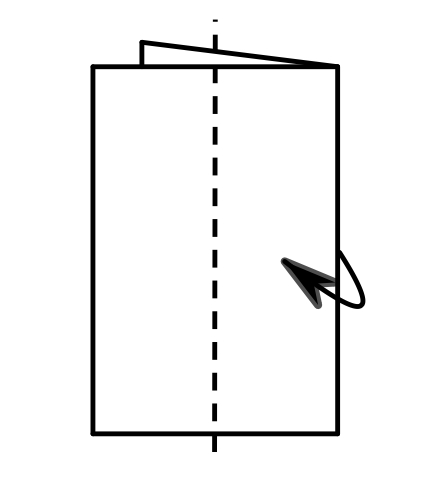
\includegraphics[width=0.3\textwidth]{./pics/Chapter_1/buchong1.png}
    \end{figure}
\end{frame}

\begin{frame}
    \frametitle{补充2}
    \textit{阴影部分是正方形,求图中最大的长方形的周长.(单位:分米)}
    \begin{figure}[H] 
        \centering
        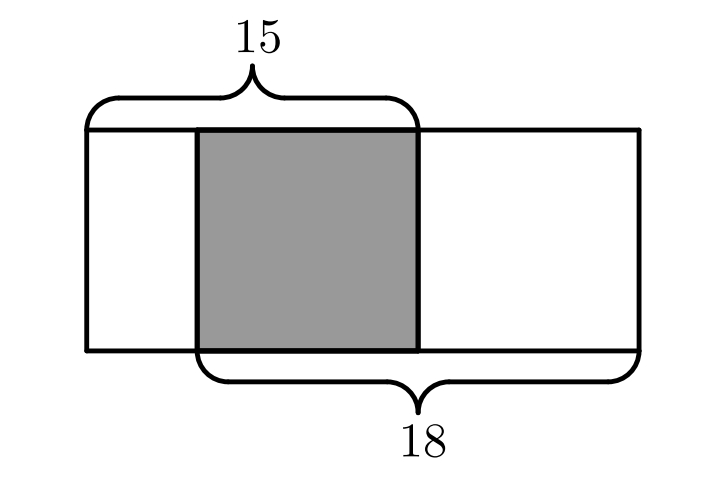
\includegraphics[width=0.5\textwidth]{./pics/Chapter_1/buchong2.png}
    \end{figure}
\end{frame}

\begin{frame}
    \frametitle{思维导图}
    \begin{figure}[H] 
        \centering
        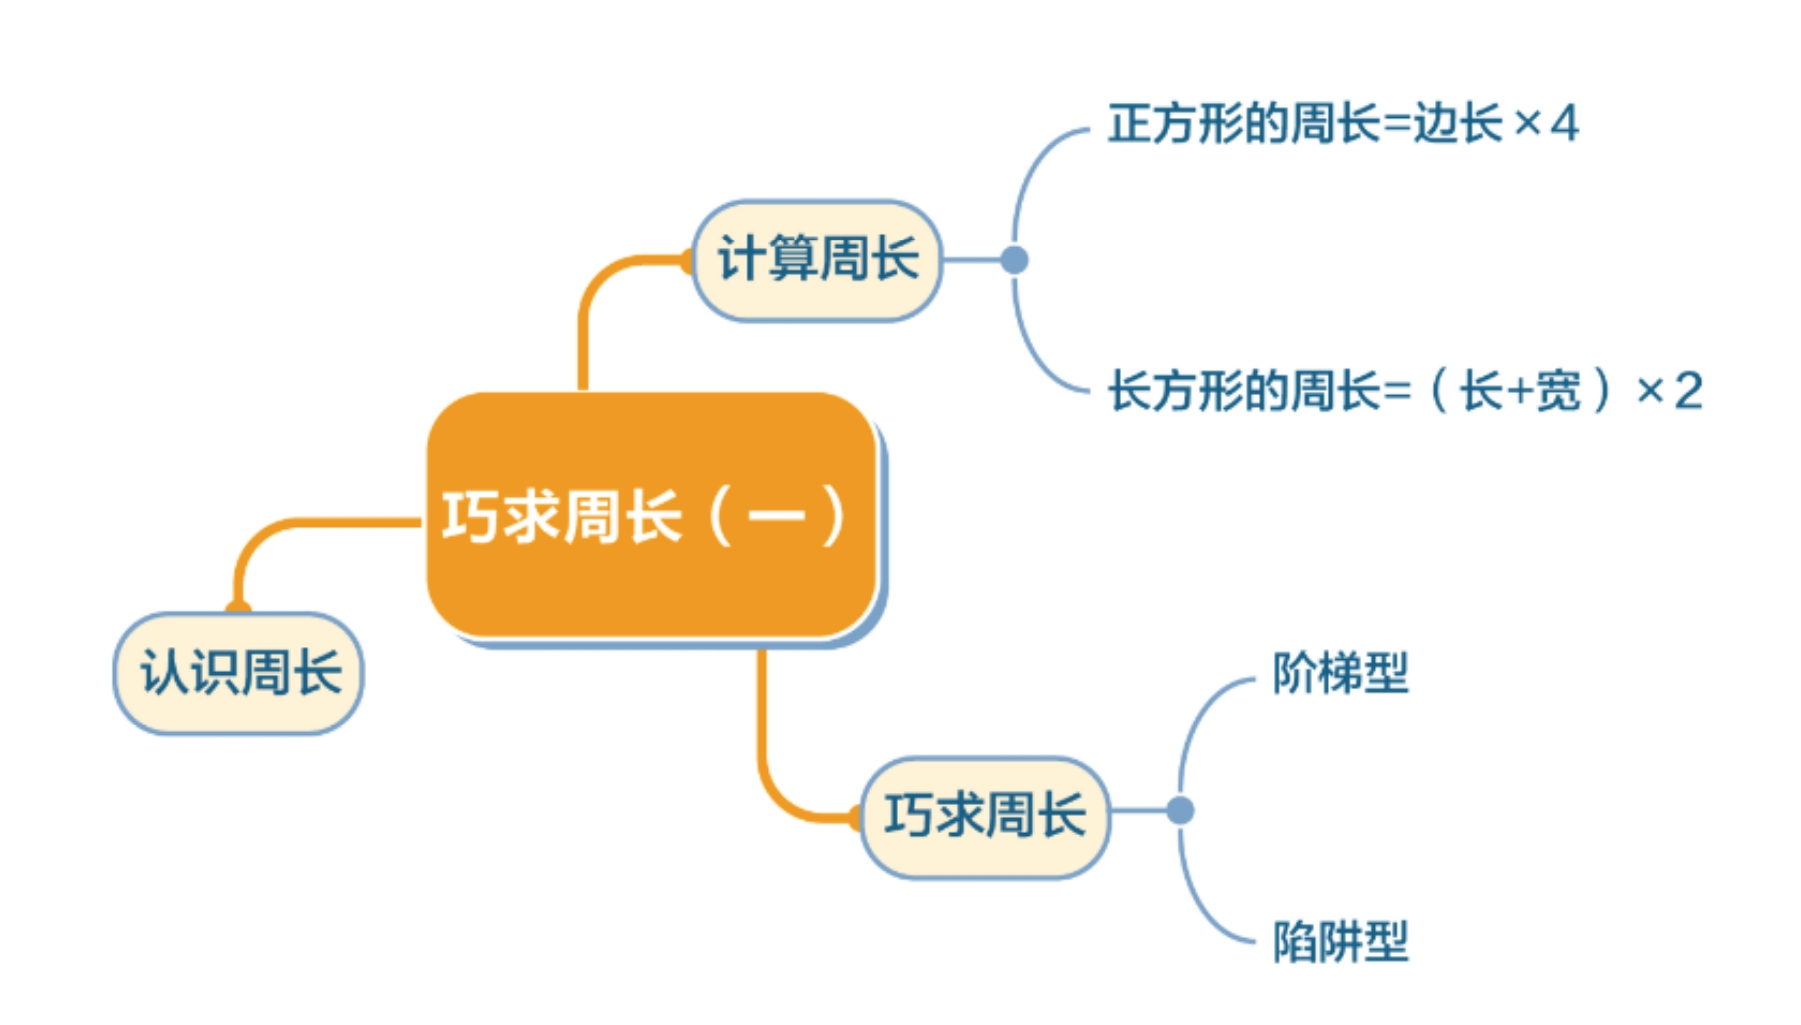
\includegraphics[width=1\textwidth]{./pics/Chapter_1/siweidaotu.png}
    \end{figure}
\end{frame}